\documentclass[]{article}
\usepackage{lmodern}
\usepackage{amssymb,amsmath}
\usepackage{ifxetex,ifluatex}
\usepackage{fixltx2e} % provides \textsubscript
\ifnum 0\ifxetex 1\fi\ifluatex 1\fi=0 % if pdftex
  \usepackage[T1]{fontenc}
  \usepackage[utf8]{inputenc}
\else % if luatex or xelatex
  \ifxetex
    \usepackage{mathspec}
  \else
    \usepackage{fontspec}
  \fi
  \defaultfontfeatures{Ligatures=TeX,Scale=MatchLowercase}
  \newcommand{\euro}{€}
\fi
% use upquote if available, for straight quotes in verbatim environments
\IfFileExists{upquote.sty}{\usepackage{upquote}}{}
% use microtype if available
\IfFileExists{microtype.sty}{%
\usepackage{microtype}
\UseMicrotypeSet[protrusion]{basicmath} % disable protrusion for tt fonts
}{}
\usepackage[margin=1in]{geometry}
\usepackage{hyperref}
\PassOptionsToPackage{usenames,dvipsnames}{color} % color is loaded by hyperref
\hypersetup{unicode=true,
            pdftitle={GVPT392(849): Introduction to GIS for Social Science Research},
            pdfauthor={Nicholas Thompson},
            pdfsubject={Mid-Term Exam},
            pdfborder={0 0 0},
            breaklinks=true}
\urlstyle{same}  % don't use monospace font for urls
\usepackage{graphicx,grffile}
\makeatletter
\def\maxwidth{\ifdim\Gin@nat@width>\linewidth\linewidth\else\Gin@nat@width\fi}
\def\maxheight{\ifdim\Gin@nat@height>\textheight\textheight\else\Gin@nat@height\fi}
\makeatother
% Scale images if necessary, so that they will not overflow the page
% margins by default, and it is still possible to overwrite the defaults
% using explicit options in \includegraphics[width, height, ...]{}
\setkeys{Gin}{width=\maxwidth,height=\maxheight,keepaspectratio}
\setlength{\parindent}{0pt}
\setlength{\parskip}{6pt plus 2pt minus 1pt}
\setlength{\emergencystretch}{3em}  % prevent overfull lines
\providecommand{\tightlist}{%
  \setlength{\itemsep}{0pt}\setlength{\parskip}{0pt}}
\setcounter{secnumdepth}{0}

%%% Use protect on footnotes to avoid problems with footnotes in titles
\let\rmarkdownfootnote\footnote%
\def\footnote{\protect\rmarkdownfootnote}

%%% Change title format to be more compact
\usepackage{titling}

% Create subtitle command for use in maketitle
\newcommand{\subtitle}[1]{
  \posttitle{
    \begin{center}\large#1\end{center}
    }
}

\setlength{\droptitle}{-2em}
  \title{GVPT392(849): Introduction to GIS for Social Science Research}
  \pretitle{\vspace{\droptitle}\centering\huge}
  \posttitle{\par}
\subtitle{Mid-Term Exam}
  \author{Nicholas Thompson}
  \preauthor{\centering\large\emph}
  \postauthor{\par}
  \predate{\centering\large\emph}
  \postdate{\par}
  \date{9am Oct3 - 5pm Oct 7, 2016}


% Redefines (sub)paragraphs to behave more like sections
\ifx\paragraph\undefined\else
\let\oldparagraph\paragraph
\renewcommand{\paragraph}[1]{\oldparagraph{#1}\mbox{}}
\fi
\ifx\subparagraph\undefined\else
\let\oldsubparagraph\subparagraph
\renewcommand{\subparagraph}[1]{\oldsubparagraph{#1}\mbox{}}
\fi


\begin{document}
\maketitle

The following coverages can be found in the PACD8 folder.

\begin{enumerate}
\def\labelenumi{\arabic{enumi}.}
\item
  PA\_CD8\_Voterfile \(=\) all registered voters for Pennsylvania,
  Congressional District 8. This is north-suburban Philadelphia,
  including all of Bucks and part of Montgomery Counties.
\item
  PA\_CD8\_Boundary \(=\) the outline for CD 8.
\item
  PA\_and\_NJ\_Counties \(=\) County boundaries for the two states.
\item
  Four States = State boundaries for PA, DE, NJ, and MD.
\item
  CD8\_PA\_Pct\_Data\_2012 \(=\) voter precinct data for 2012.
\item
  Mont\_County\_Recent\_Movers\_10\_12.
\item
  Bucks\_County\_Recent\_Movers\_10\_12.
\item
  CD8\_Places.
\item
  PA CD8\_Tracts.
\end{enumerate}

Three files above contain points for voters at their residences. These
are 1, 6, and 7. For these files, the following columns contain
important information:

Age (and Year Born) \(=\) the age of the voter in 2012.

Rep\_Party, Dem\_Party, Ind\_Unaf\_Party \(=\) the party registration of
the voter: Rep \(=\) Republican, Dem \(=\) Democratic, and Ind\_Unaf
\(=\) Independent/Unaffiliated.

And there are other items that will be less important for this exercise.

\begin{center}\rule{0.5\linewidth}{\linethickness}\end{center}

For the following questions, use whatever tools you deem appropriate
form the ArcGIS package, but be sure to describe what you did to address
the questions. Be resourceful, but you need not write more than one page
in response to each question.

\begin{enumerate}
\def\labelenumi{\arabic{enumi}.}
\tightlist
\item
  Aggregate the voter and mover data to the census tract level for PA
  CD8.
\end{enumerate}

~~~~~~To aggregate the data, I used a three phase process with multiple
steps in each phase. In Phase 1, I imported the data using the catalogue
in ArcMap. To import the data I first created a geodatabase file named
\texttt{exam}. Here I imported all exam shapefiled included in the
provided exam folder by right clicking on the \texttt{exam.gdb} and
selecting import from multiple. Next I systemtaically added four file
layers to the ArcMap table of contents:

~~~~~~a. PA\_CD8\_Voterfile (hereafter depicted as \texttt{voter});

~~~~~~b. Mont\_County\_Recent\_Movers\_10\_12 (hereafter depicted as
\texttt{MC});

~~~~~~c. Buck\_County\_Recent\_Movers\_10\_12 (hereafter depicted as
\texttt{BC});

~~~~~~d. PA\_CD8\_Tracts (hereafter depicted as \texttt{tracts}).

This was the end of Phase 1.

~~~~~~In Phase 2, I reviewed the data and deleted unnecessary fields.
The number is too great to depict which were removed. I kept essential
fields outlined in the instructions above, as well as some others that I
anticipated would be necessary (including \texttt{MOVER} from the
\texttt{voter} file, \texttt{ozipcode} and \texttt{dzipcode} from
\texttt{MC} and \texttt{BC}, and \texttt{ORNIC}, \texttt{DRNIC}, and
\texttt{RNIC} from \texttt{voter}, \texttt{BC}, and \texttt{MC}). The
combination of fields chosen allowed me to manipulate the data to
achieve the desired results. I removed fields by double-clicking on each
layer in the table of contents and navigating to the \texttt{Fields}
tab. After clearing all of the fields, I was able to check only the
fields I wanted to keep. Next, I exported the data into new layers
within the geodatabase. This data management process ended Phase 2.

~~~~~~In Phase 3, I used the \texttt{Spatial\ Join} feature (hereafter
known as \texttt{SJ}) to systemtaically join the layers. First I
conducted a \texttt{SJ} of \texttt{voters} to \texttt{tracts} and
created a new layer called \texttt{tracts05}. Next I created the
following \texttt{SJ}s:

~~~~~~a. \texttt{BC} \(+\) \texttt{tracts} \(=\) \texttt{tracts04}

~~~~~~b. \texttt{MC} \(+\) \texttt{tracts} \(=\) \texttt{tracts06}

~~~~~~c. \texttt{tracts05} \(+\) \texttt{tracts04} \(=\)
\texttt{tracts09}

~~~~~~d. \texttt{tracts09} \(+\) \texttt{tracts06} \(=\)
\texttt{tracts15}

The last combination created a spatially joined dataset depicting the
north-suburban part of Philadelphia.

\begin{itemize}
\tightlist
\item
  Then compute and calculate the Democratic \(\%\) of total registered
  voters (10 points).
\end{itemize}

To compute and calculate the Democratic \(\%\) of total registered
voters I needed to create a new field in the \texttt{BC} and \texttt{MC}
shapefiles. I completed these computations prior to merging all of the
data to ensure that they were carried over in each of the \texttt{SJ}s.
First, I created a new field called \texttt{vote\_total}. Using the
field calculator tool, I added the \texttt{Republican},
\texttt{Democratic}, and \texttt{Independent} fields together. This
produced a one in each row of the \texttt{vote\_total}. Next, I used the
statistics tool to calculate the total sum of from the
\texttt{Democratic} field and the the sum from the \texttt{vote\_total}
fields. I conducted statistical analysis before and after conducting the
joins. The Table 1 below shows the outcomes. Note there is no
significant difference in the percentages either pre- or post-join.

\begin{table}[]
\centering
\caption{Percentage of Democratic Voters}
\begin{tabular}{lll}
Field       & Pre-Join & Post-Join \\
\hline
Democratic  & 71,048   & 133,467   \\
vote\_total & 540,451  & 1,019,887 \\
\hline
\hline
Percentages & 53.23 \% & 52.99 \% 
\end{tabular}
\end{table}

\begin{itemize}
\item
  Compute and calculate the Democratic \(\%\) of total movers in Bucks
  and Montgomery counties (10 points).
\item
  Produce two maps of these percentages.
\end{itemize}

\begin{figure}[htbp]
\centering
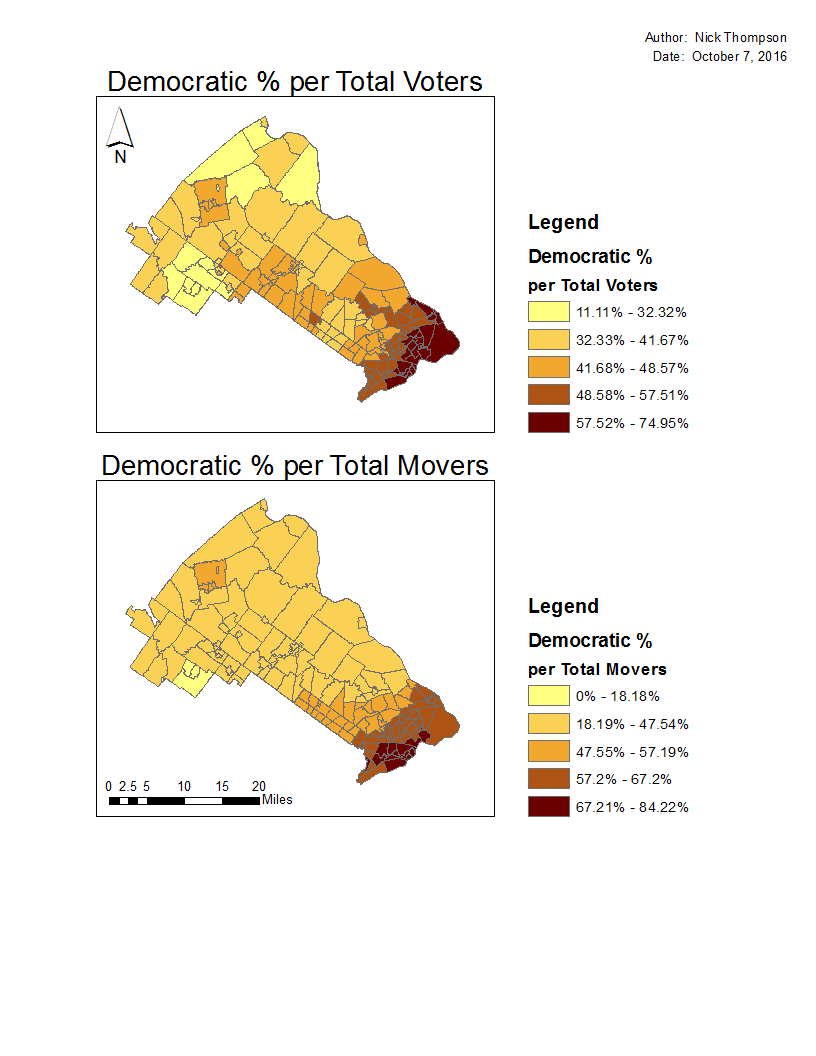
\includegraphics{question_1.png}
\caption{Democratic Voter Percentages}
\end{figure}

\end{document}
